\documentclass[12pt,a4paper]{article}

% Pacote para exibição de imagem
\usepackage{graphicx}

% Onde buscar imagem
\graphicspath{{./img/}}

\title{Unidade II: Modelagem de Dados}
\author{Fernando de Lima Gonçalves}
\date{\today}

%\overfullrule=5pt

\begin{document}
\maketitle

\section{Conceitos}
\begin{description}
    \item[\textbf{Modelo de Dados}:] 
        \sloppy é uma coleção de ferramentas conceituais para descrição dos dados e  
        seus relacionamentos, restrições de consistência e semântica.
    \item[\textbf{Modelagem de Dados}:] método de análise que, a partir de fatos relevates a um contexto de negócio, 
        determina a perspectiva dos dados, permitindo organizá-los em estruturas bem definidas e estabelecer regras de dependência.
    \item[\textbf{Modelos de BD}:]\hfill
        \begin{itemize}
            \item Hierárquico
            \item Rede
            \item Relacional
            \item Pós-Relacionais
            \item Orientados a Objeto
        \end{itemize}
\end{description}

\section{Modelo de Entidades-Relacionamentos}
\begin{itemize}
    \item O Modelo E-R é um tipo de \textit{Modelo Conceitual} baseado na percepção do mundo real.
    \item O Modelo E-R é uma forma de representar os requisitos funcionais levantados durante a fase de análise.
    \item O Modelo E-R possui grande capacidade semântica, facilitando a compreensão pelo usuário leigo e a validação dos dados de aplicação a ser modelada.
\end{itemize}

\subsection{Entidades}
\begin{itemize}
    \item Objetos do mundo real como: \textit{\textbf{Clientes, Funcionários, Produtos, etc.}}
    \item Estruturas abstratas como: \textit{\textbf{Nota fiscal, histórico escolas, extratos, etc.}}
    \item A entidade é representada por um \textbf{\textit{\underline{retângulo nomeado}}} substantivo que designa todo um conjunto de instâncias similares como:\par Pedro e Paulo são instâncias da Entidade \textit{\textbf{Cliente}}
\end{itemize}

\subsubsection{Atributos}
\begin{itemize}
    \item Elementos de dados que identificam e descrevem Entidades
        \begin{itemize}
            \item \textbf{Ex:} Fornecedor = cod-fornecedor, nome, CNPJ, etc.
        \end{itemize}
    \item Dado que é assoociado a cada ocorrência de uma entidade ou relacionamento
    \item É representado por uma \textbf{\textit{\underline{elipse nomeada}}}
    \item Podem ser de vários tipos:
        \begin{description}
            \item[\textbf{Simples:}] indivisíveis como: CPF, preço, altura, etc.
            \item[\textbf{Composto:}] divisíveis em subpartes menores, independentes e que podem formar uma hierarquia.
                \begin{itemize}
                    \item \textbf{Ex:} Cód. do País + Cód. do Estado + Número de Telefone
                \end{itemize}
        \end{description}
\end{itemize}

\subsubsection{Tipos de Atributos}
\begin{description}
    \item[\textbf{Monovalorados:}]
        possuem um único valor para uma dada entidade.
        \begin{itemize}\item \textbf{Ex:} CPF, nome, altura e peso de uma pessoa.\end{itemize}
    \item[\textbf{Multivalorados:}]
        múltiplos valores para uma dada entidade, representado por uma \textit{\textbf{\underline{elipse dupla}}}
        \begin{itemize}
            \item \textbf{Ex:} Telefones e Endereços de fornecedores.
        \end{itemize}
    \item[\textbf{Derivados:}] computados a partir de outros atributos ou entidades. Representado por uma \textbf{\textit{\underline{elipse pontilhada}}}
        \begin{itemize}
            \item \textbf{Ex:} Idade do Aluno, Índice de Massa Corporal (IMC), Total da nota Fiscal.
        \end{itemize}
\end{description}

\newpage % Quebra de página -> Manter formatação

\subsubsection{Atributo Chave}

\begin{itemize}
    \item Atributos cujos valores são distintos nas ocorrências da entidade.
    \item É uma restrição de unicidade (exclusividade).
    \item Identificador da entidade
    \item É representado por uma \textbf{\textit{\underline{elipse nomeada de texto sublinhado}}}
        \begin{itemize}
            \item \textbf{Ex:} CPF de pessoa, Código do voo, CNPJ da empresa
        \end{itemize}
    \item Uma entidade pode ter mais de um atributo chave
        \begin{itemize}
            \item \textbf{Ex:} CPF e número de matrícula do Aluno
        \end{itemize}
    \item Chave composta: quando vários atributos formam uma chave
        \begin{itemize}
            \item número de nota fiscal + número do item
            \item Número da agência + número da conta
        \end{itemize}
\end{itemize}

\subsection{Relacionamentos}

\subsubsection{Cardinalidade}

\begin{itemize}
    \item
        Associação entre uma ou várias entidades com determinado significado.
    \item
        Conjunto de associações entre ocorreências de entidades representados por um \textit{\textbf{\underline{losango nomeado}}}
    \item \begin{description}
            \item[\textbf{Cardinalidade:}] 
                propriedade do relacionamento que expressa o nú\-me\-ro de ocorrências de uma entidade que participa do relacionamento com outra(s) entidade(s).
                \begin{itemize}
                    \item \textbf{Um-para-Um}: Técnico e Time
                    \item \textbf{Um-para-Muitos}: Proprietário e Veículo
                    \item \textbf{Muitos-para-Um}: Veículo e Proprietário
                    \item \textbf{Muitos-para-Muitos}: Paciente e Médico, Professor e Aluno
                \end{itemize}
     \end{description}
     \item \begin{description}
             \item[\textbf{Totalidade:}]: é uma propriedade que especifica se a existência de uma entidade depende de seu relationamento com outra entidade.
                 \begin{itemize}
                     \item pode ser \textbf{parcial} \textit{(opcional)} ou \textbf{total} \textit{obrigatório}.
                     \item \textbf{Ex:} Sócio e Dependente
                 \end{itemize}
         \end{description}
     \item É fundamental consultar o usuário sobre as regras de negócio para as \textit{cardinalidades} e \textit{totalidade}.
\end{itemize}

\newpage

\subsubsection{Relacionamentos Recursivos}
\begin{itemize}
    \item
        Uma ocorrência de uma entidade se relaciona com outra(s) corrência(s) da mesma entidade.
    \item 
        A mesma entidade participa mais de uma vez em um tipo de relacionamento em \textbf{papéis} diferentes
        \begin{itemize}
            \item
                \textbf{Ex:} Uma disciplina tem um ou vários pré-requisitos de outras disciplinas, uma música pode possuir várias versões que também são músicas.
        \end{itemize}
\end{itemize}

\subsection{Conceitos Avançados do M.E.R}
\begin{itemize}
    \item \textbf{Entidade forte e Entidade fraca}
    \item \textbf{Atributos de Relacionamento}
    \item \textbf{Relacionamentos Binários e Ternários}
    \item \textbf{M.E.R. Estendido: Generalizações e Especialização}
\end{itemize}

\subsubsection{Entidades Fracas}
\begin{itemize}
    \item Tipos de entidade que não têm chave própria
    \item As instâncias são identificadas por meio do relacionamento com entidades de outro tipo (identificador), juntamento com os valores de alguns atributos (chave parcial)
    \item Precisa da entidade forte para definis sua identidade
    \item Representada por um \textbf{\textit{\underline{Retângulo Duplo}}}
\end{itemize}

\newpage\subsection{Grau de Relacionamento: Binários e Ternários}
\begin{itemize}
    \item
        Número de tipos de entidades participantes de um tipo de re\-la\-cio\-na\-men\-to.
    \item
        Na maioria das vezes, os relacionamentos são \textbf{binários} (grau 2).
    \item 
        As entidades participantes atuam com \textbf{\textit{papel}} determinado no relacionamento.
\end{itemize}

\begin{figure}[h]
    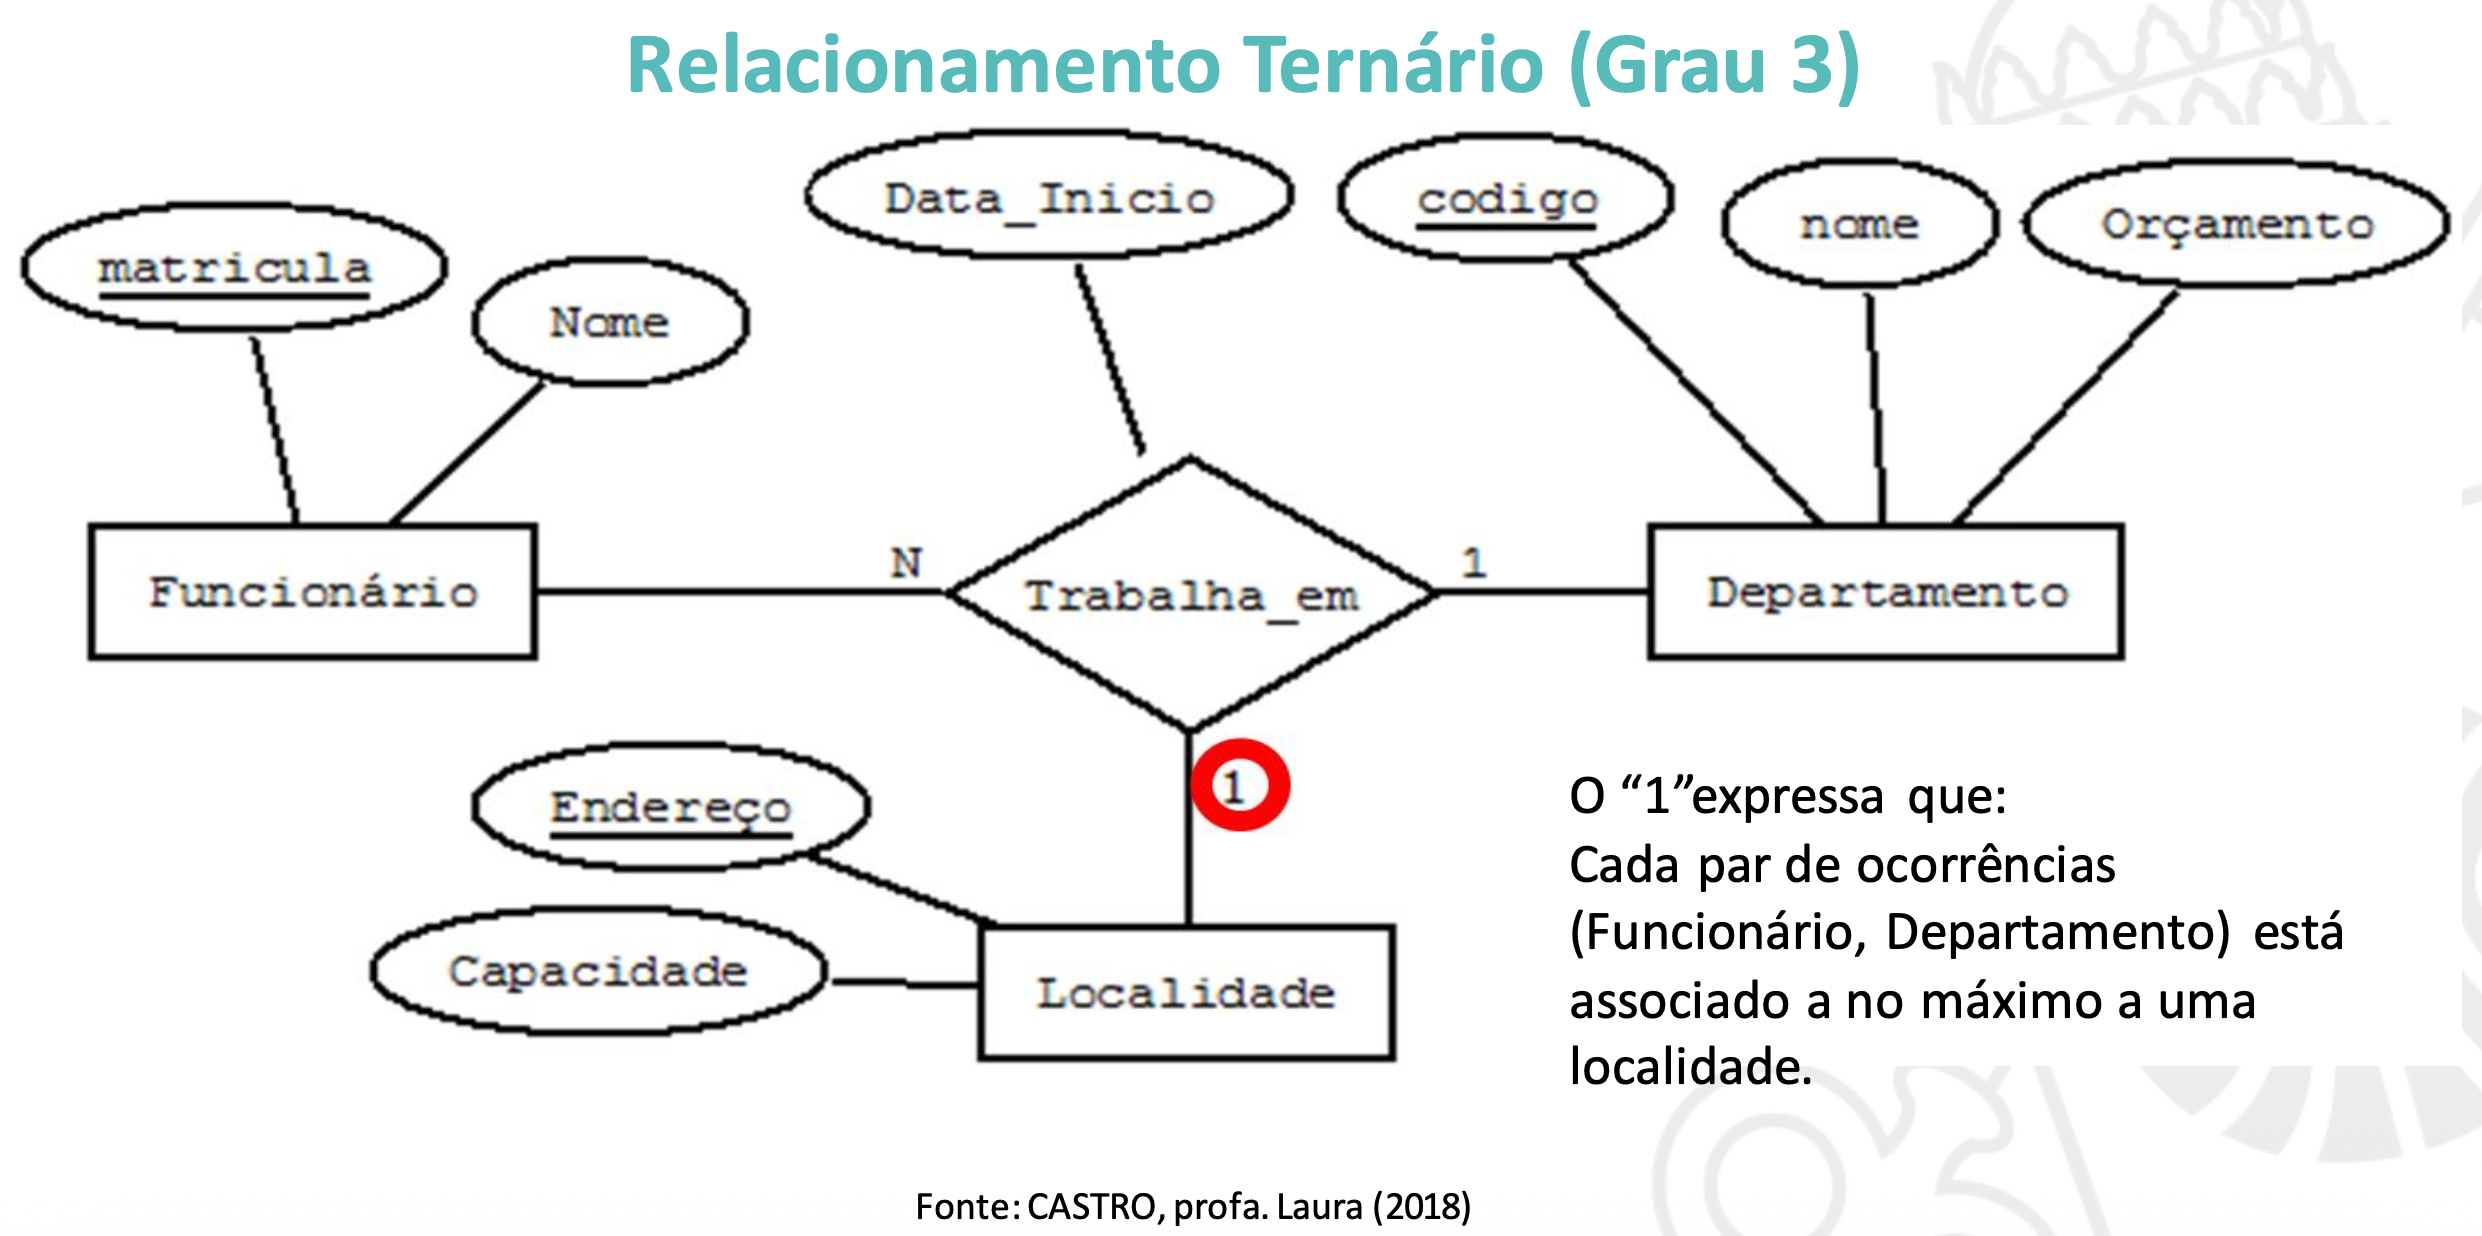
\includegraphics[width=\linewidth, height=\textheight, keepaspectratio]{Relacionamento-Ternario}
\end{figure}

\newpage\subsection{MER Estendido: Generalização e Especialização}
\begin{description}
    \item[\textbf{Generalização}:] 
        Processo de definição de entidade genérica (super-classe ou super-tipo)
        \begin{itemize}
            \item \textbf{Ex:} Pessoa é generalização de Pessoa Física e Pessoa Jurídica
        \end{itemize}
    \item[\textbf{Especialização}:] 
        Processe de definição de subclasses de uma entidade
        \begin{itemize}
            \item \textbf{Ex:} Cliente especial é especialização de Cliente
        \end{itemize}
\end{description}
\begin{itemize}
    \item Uma entidade de um subtipo \textbf{herda} todos os atributos e relacionamentos de seu super-tipo.
    \item Uma entidade de um subtipo pode ou não possuir atributos próprios e relacionamentos específicos
\end{itemize}

\begin{figure}[h]
    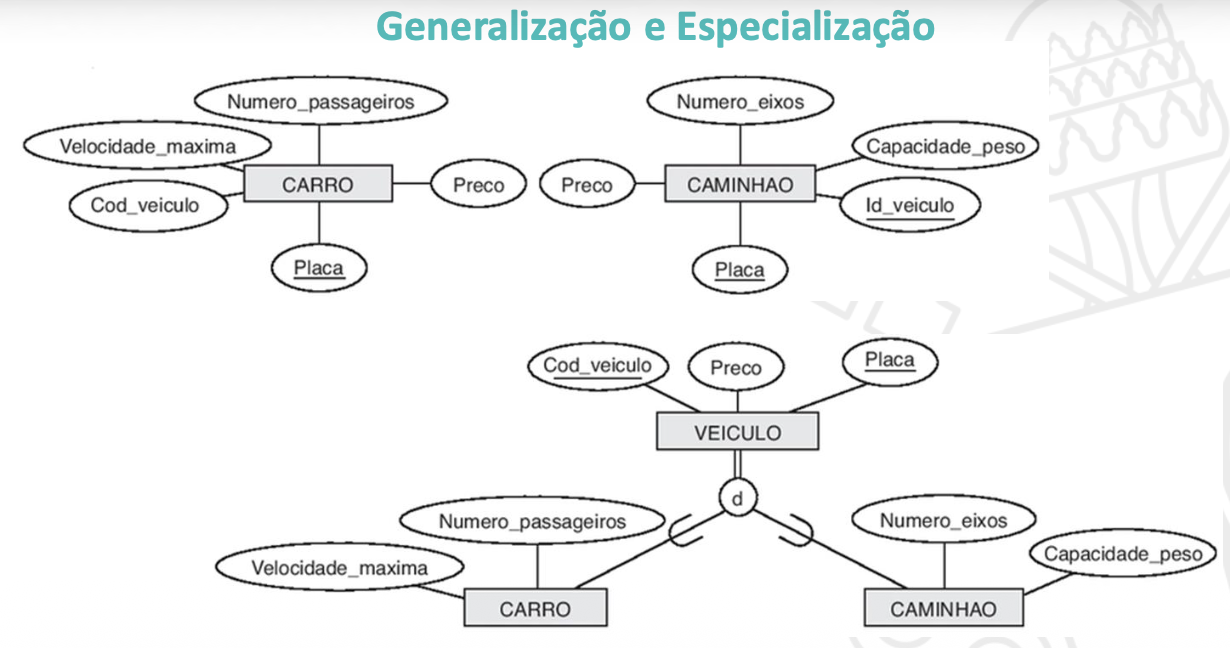
\includegraphics[width=\linewidth,height=\textheight,keepaspectratio]{subtipos}
\end{figure}

\newpage
\begin{itemize}
    \item \textbf{Disjunção}: subtipos podem ser \textbf{\textit{disjuntos}} ou \textbf{\textit{sobrepostos}}
        \begin{itemize}
            \item \textbf{\underline{Disjunto}}
                \begin{itemize}
                    \item entidade de supertipo pode pertencer a \textbf{APENAS UM} subtipo de especialização.
                    \item representado pela letra \textbf{b} ciculada.
                \end{itemize}
            \item \textbf{\underline{Sobreposto}}
                \begin{itemize}
                    \item entidade de supertipo pode pertencer a \textbf{VÁRIOS} subtipos.
                    \item representado pela letra \textbf{s} \textbf{o} ciculada.
                \end{itemize}
        \end{itemize}
    \item \textbf{Completude:} completudo do super-tipo aos subtipos pode ser \textbf{\textit{total}} ou \textbf{\textit{parcial}}.
        \begin{itemize}
            \item \textbf{Parcial:}
                \begin{itemize}
                    \item entidades \textbf{PODEM NÃO} pertencer a algum subtipo.
                    \item Representado por \textbf{\textit{linha simples}}.
                \end{itemize}
            \item \textbf{Total:}
                \begin{itemize}
                    \item entidades \textbf{DEVEM} pertencer a, pelo menos, um subtipo.
                    \item Representado por \textbf{\textit{linha dupla}}.
                \end{itemize}
        \end{itemize}
    \item \textbf{Combinações Possíveis:}
        \begin{itemize}
            \item Disjunto / Total
            \item Disjunto / Parcial
            \item Sobreposto / Total
            \item Sobreposto / Parcial
        \end{itemize}
\end{itemize}

\newpage
\begin{figure}[h]
    %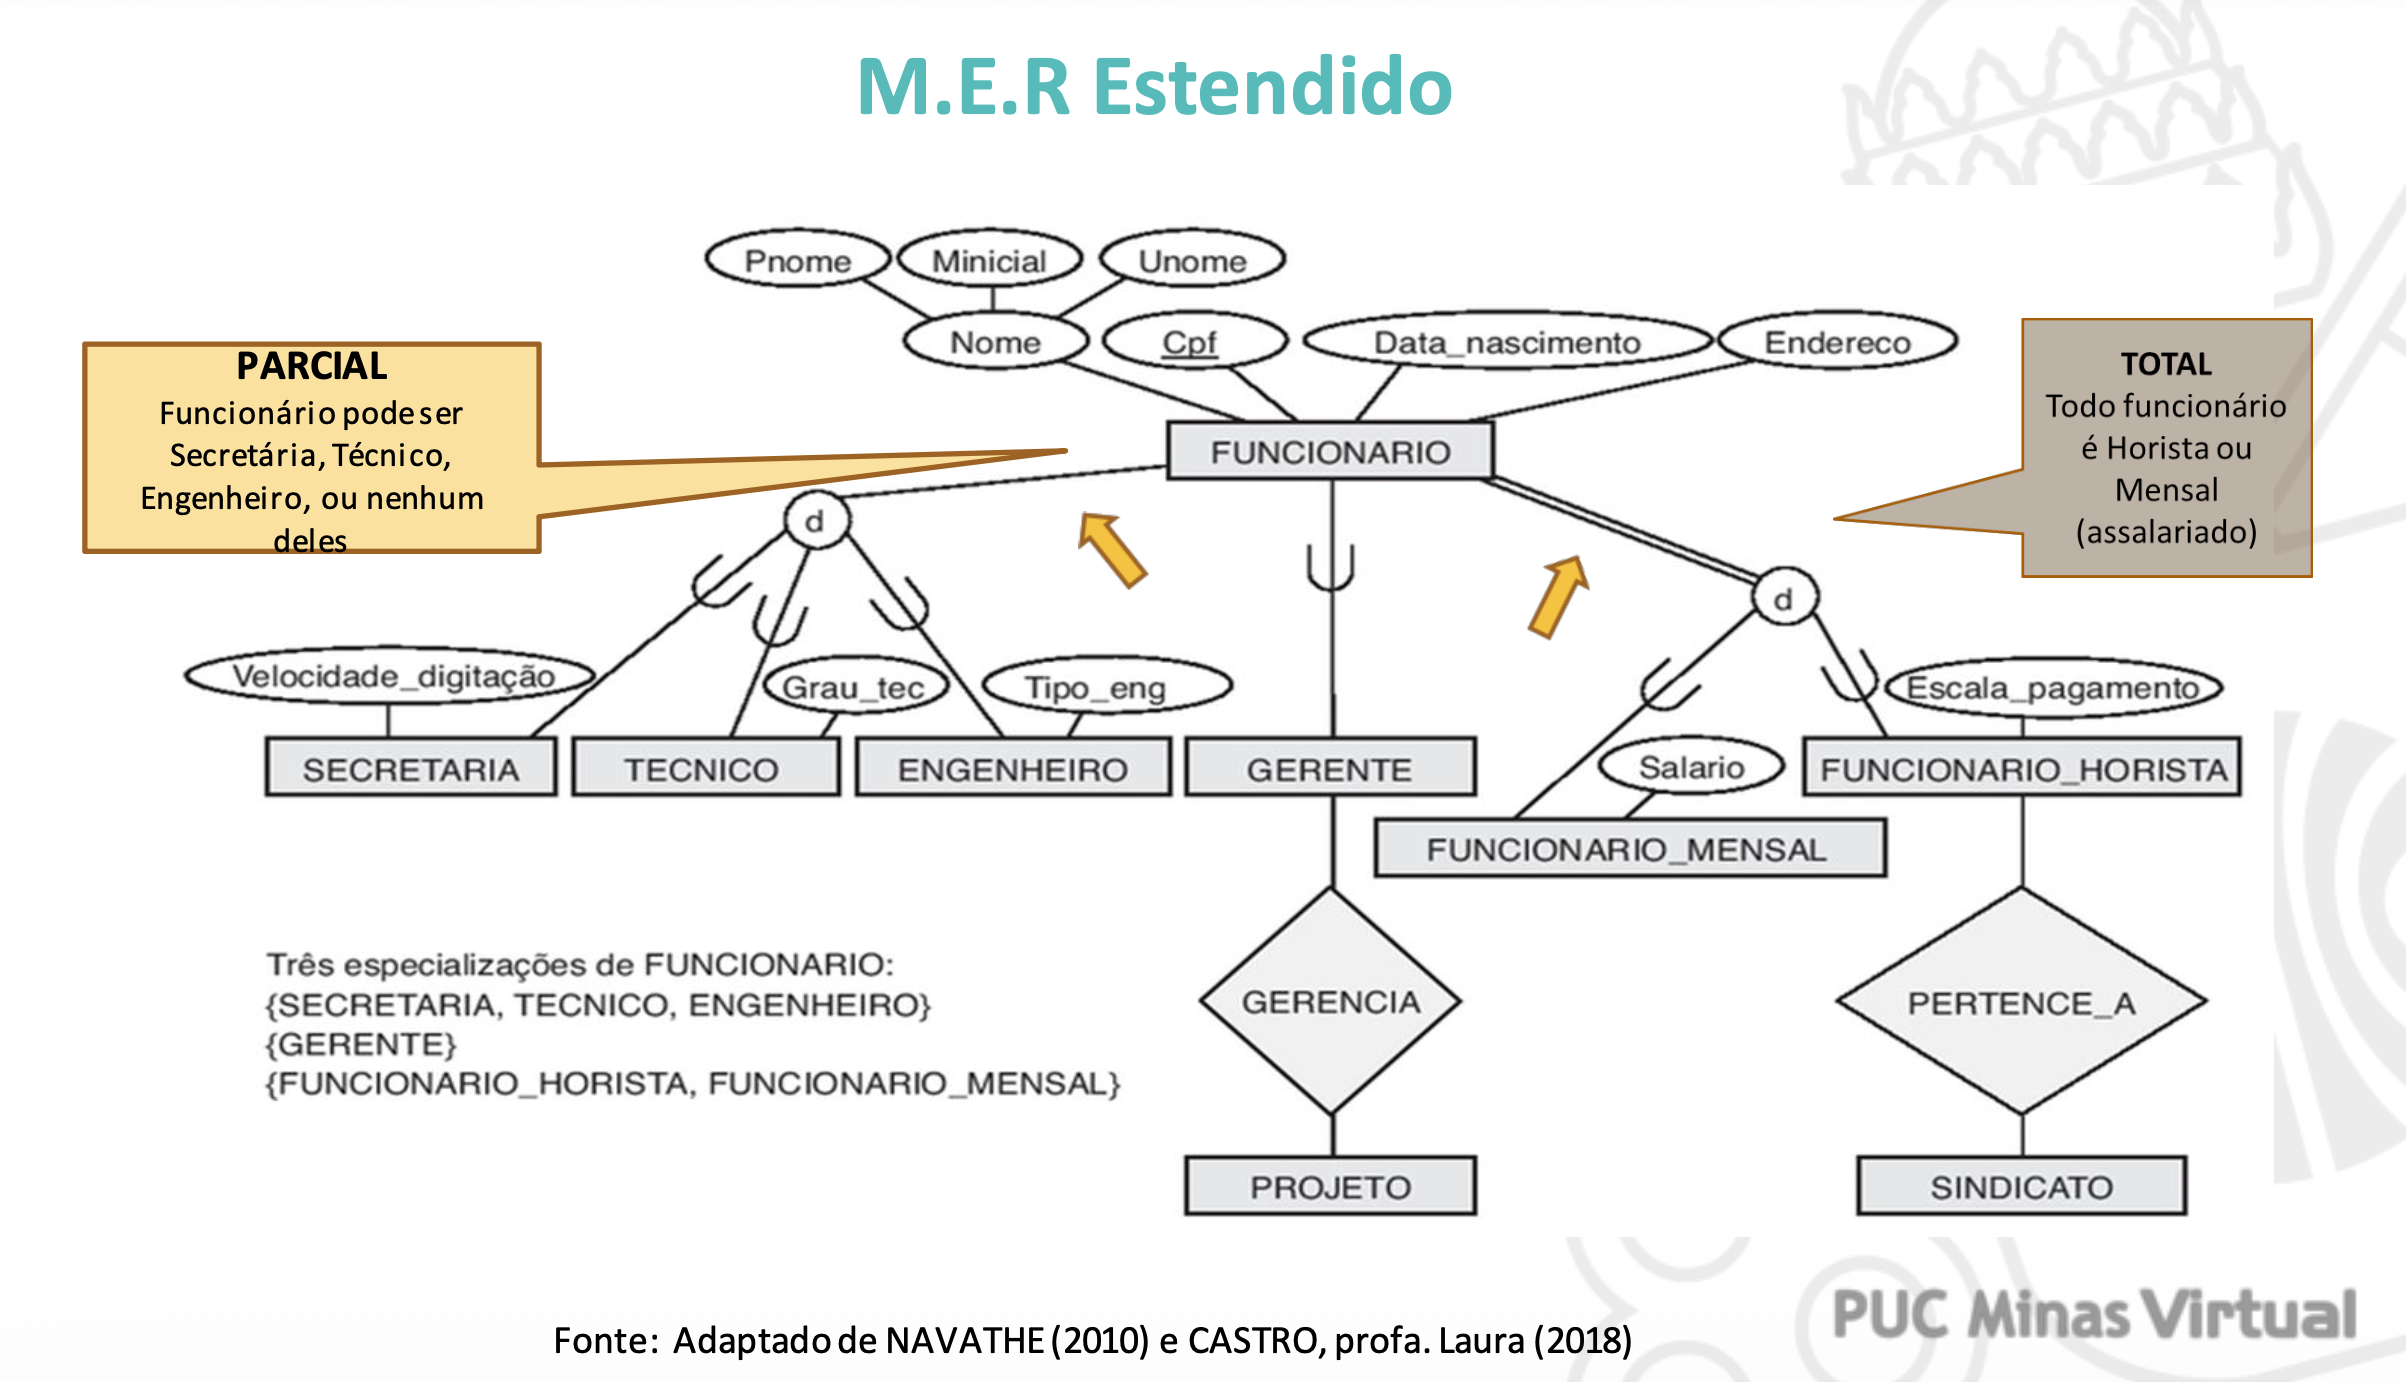
\includegraphics[scale=0.2]{MER-estendido}
    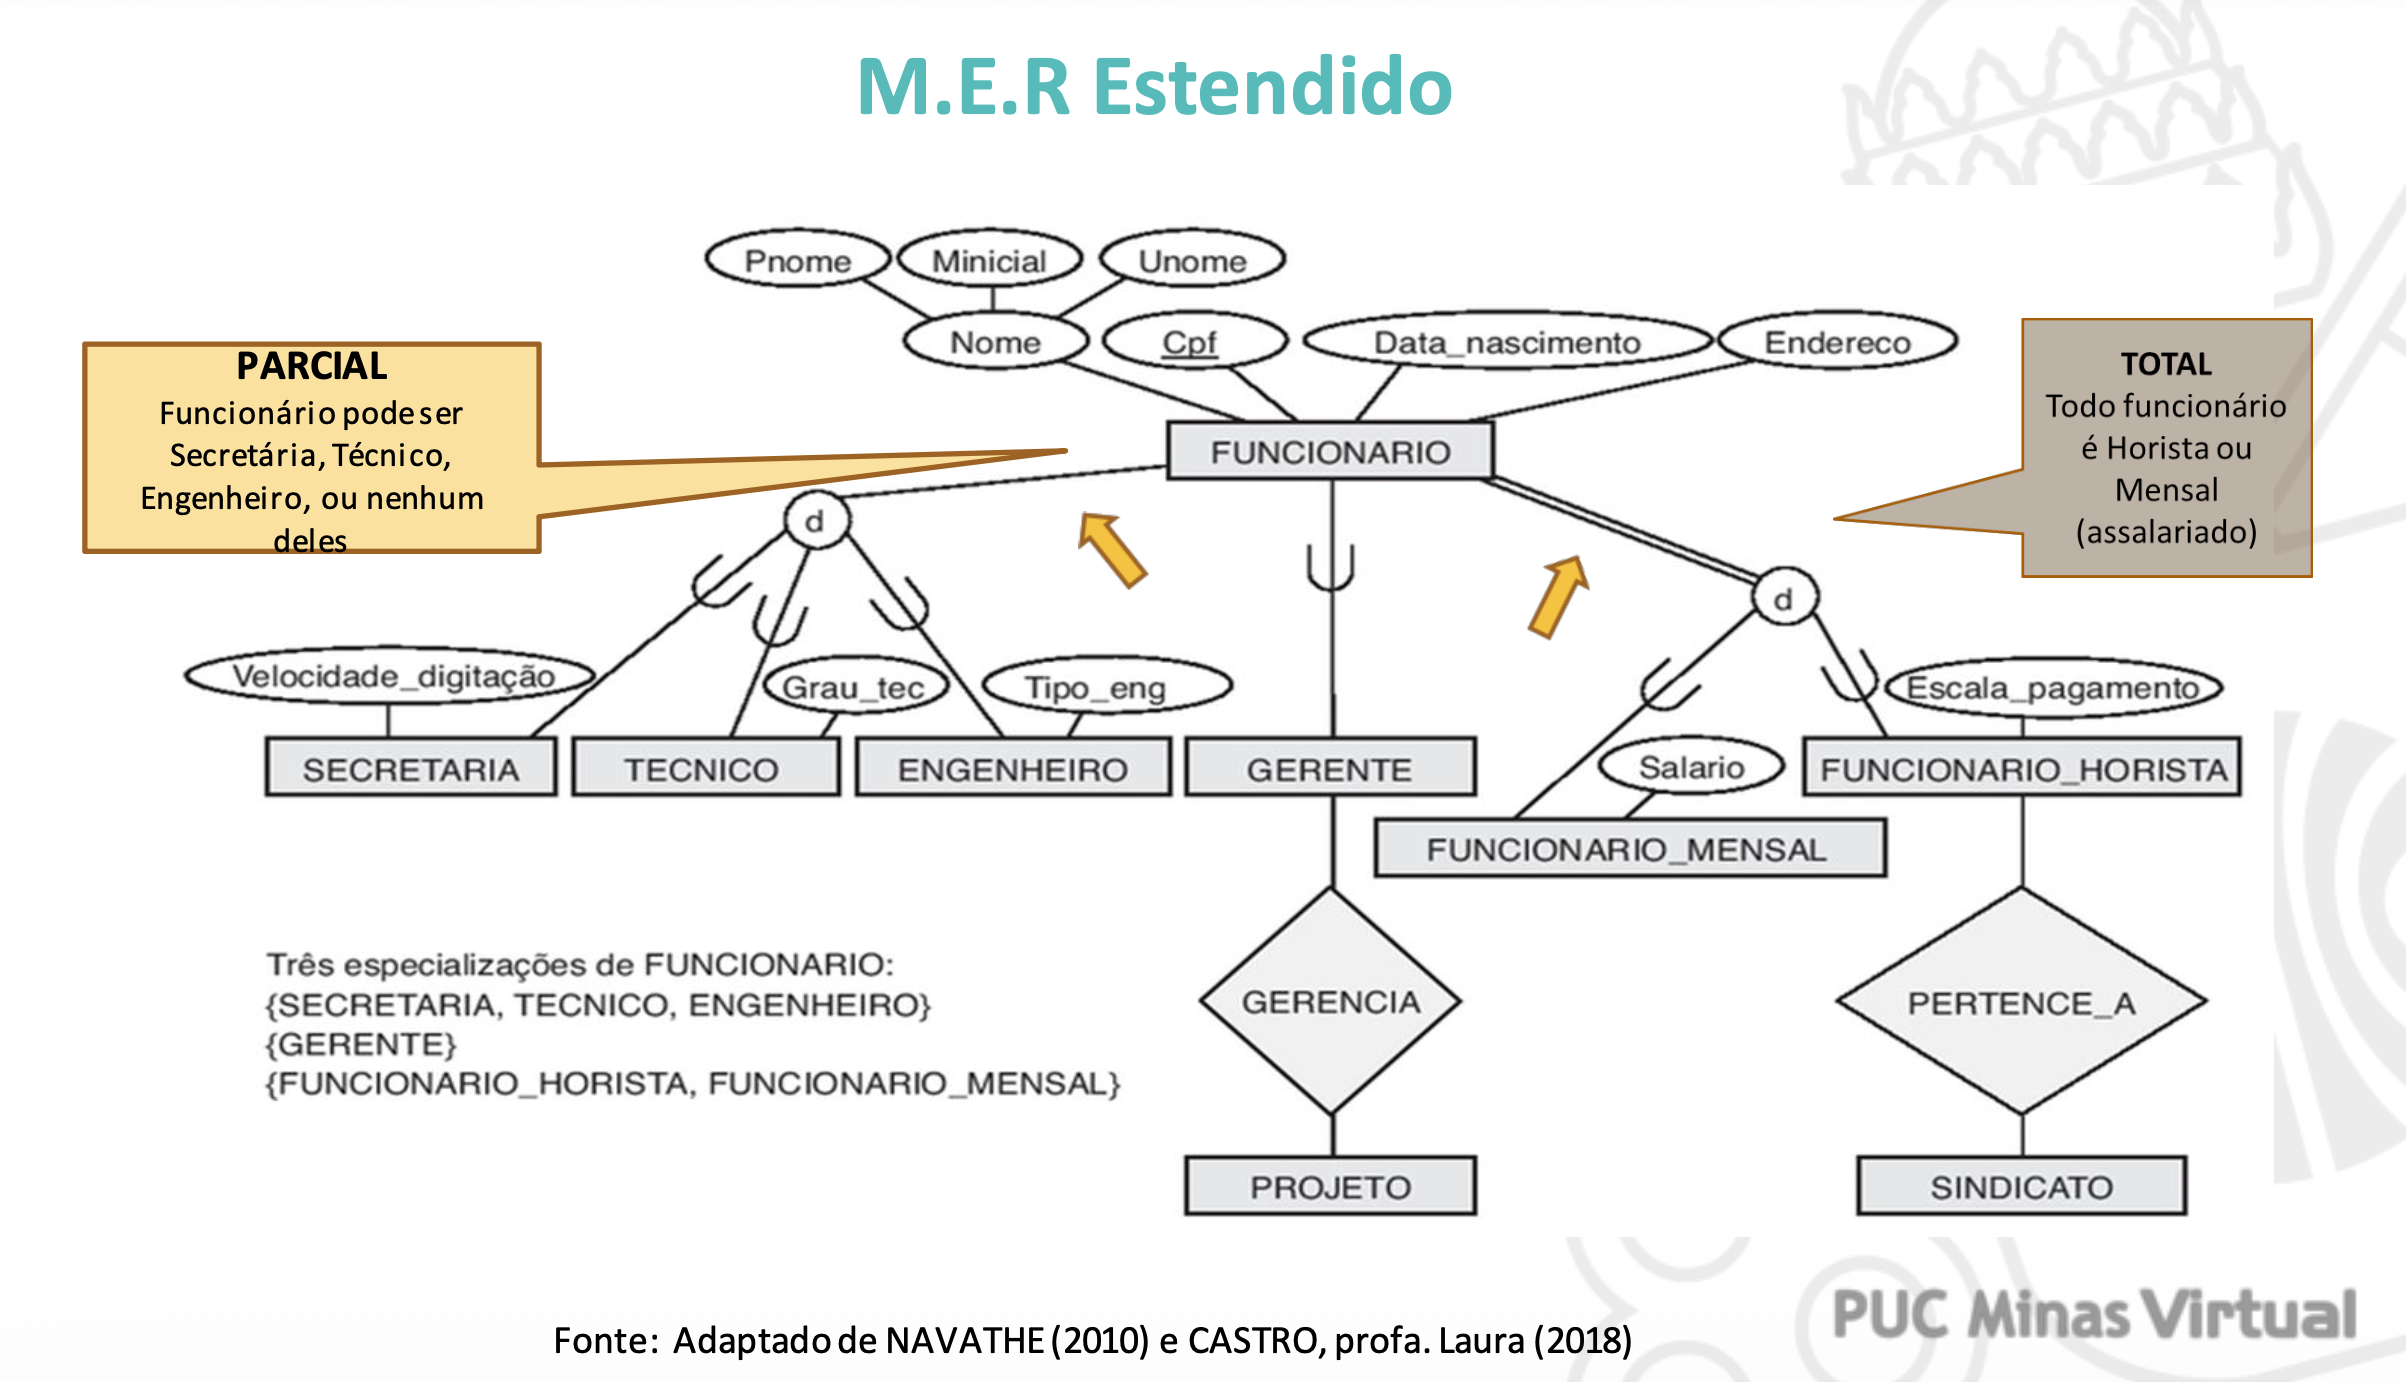
\includegraphics[width=\linewidth,height=\textheight,keepaspectratio]{MER-estendido}
\end{figure}

\end{document}
